%%% Для сборки выполнить 2 раза команду: pdflatex <имя файла>

\documentclass[a4paper,12pt]{article}

\usepackage{ucs}
\usepackage[utf8x]{inputenc}
\usepackage[russian]{babel}
%\usepackage{cmlgc}
\usepackage{graphicx}
\usepackage{listings}
\usepackage{xcolor}
%\usepackage{courier}

\makeatletter
\renewcommand\@biblabel[1]{#1.}
\makeatother

\newcommand{\myrule}[1]{\rule{#1}{0.4pt}}
\newcommand{\sign}[2][~]{{\small\myrule{#2}\\[-0.7em]\makebox[#2]{\it #1}}}

% Поля
\usepackage[top=20mm, left=30mm, right=10mm, bottom=20mm, nohead]{geometry}
\usepackage{indentfirst}

% Межстрочный интервал
\renewcommand{\baselinestretch}{1.50}


\begin{document}

%%%%%%%%%%%%%%%%%%%%%%%%%%%%%%%
%%%                         %%%
%%% Начало титульного листа %%%

\thispagestyle{empty}
\begin{center}
\renewcommand{\baselinestretch}{1}
\large
{\sc Министерство образования и науки Российской Федерации\\
ФГБОУ <<Петрозаводский государственный университет>>\\
Институт математики и информационных технологий\\
Кафедра информатики и математического обеспечения}

\end{center}

\vfill

\begin{center}
{\normalsize Промежуточный отчет о научно-исследовательской работе} \\

\medskip

%%% Название работы %%%
{\Large \sc Мобильное приложение персонализированный трекер пользователя}
\end{center}

\medskip

\begin{flushright}
\parbox{11cm}{%
\renewcommand{\baselinestretch}{1.2}
\normalsize
Выполнил:\\
%%% ФИО студента %%%
студент 2 курса группы 22207 В. В. Клименко
\begin{flushright}
\sign[подпись]{4cm}
\end{flushright}

Научный руководитель:\\
%%% степень, звание ФИО научного руководителя %%%
к.ф.-м.н., преподаватель В. М. Димитров\\
Оценка руководителя:\hfill\rule{4cm}{0.4pt}
\begin{flushright}
\sign[подпись]{4cm}
\end{flushright}

Представлен на кафедру
\begin{flushright}
  <<~\myrule{0.8cm}~>>~\myrule{4cm}~~2018~г.\\[1em]
  \sign[подпись принявшего работу]{6cm}
\end{flushright}
}
\end{flushright}

\vfill

\begin{center}
\large
Петрозаводск --- 2018
\end{center}

%%% Конец титульного листа  %%%
%%%                         %%%
%%%%%%%%%%%%%%%%%%%%%%%%%%%%%%%
\pagebreak
%%%%%%%%%%%%%%%%%%%%%%%%%%%%%%%%
%%%                          %%%
%%% Содержание               %%%

\newpage

\tableofcontents


%%% Содержание              %%%
%%%                         %%%
%%%%%%%%%%%%%%%%%%%%%%%%%%%%%%%

\pagebreak

%%%%%%%%%%%%%%%%%%%%%%%%%%%%%%%%
%%%                          %%%
%%% Введение                 %%%

%%% В введении Вы должны описать предметную область, с которой связана %%%
%%% Ваша работа, показать её актуальность, вкратце определить цель     %%%
%%% исследования/разработки					       %%%

\section*{Введение}
\addcontentsline{toc}{section}{Введение}

Трекер - это программа позволяющая отслеживать путь пользователя и выводить
различную информацию о том, каким образом он перемещался.

Сегодня такое приложение необходимо тем, кто занимается туризмом и спортом.
Ведь это очень удобно, чтобы человек имел статистику о том, с какой скоростью,
где и сколько он прошёл. Однако пользователь вынужден включать и выключать 
запись своих передвижений, что уменьшает удобность использования.
Целью данной работы является создание трекера, котрый работал бы в фоновом режиме,
то есть постоянно вёл запись перемещений без участия пользователя.

\begin{figure}
	\centering
	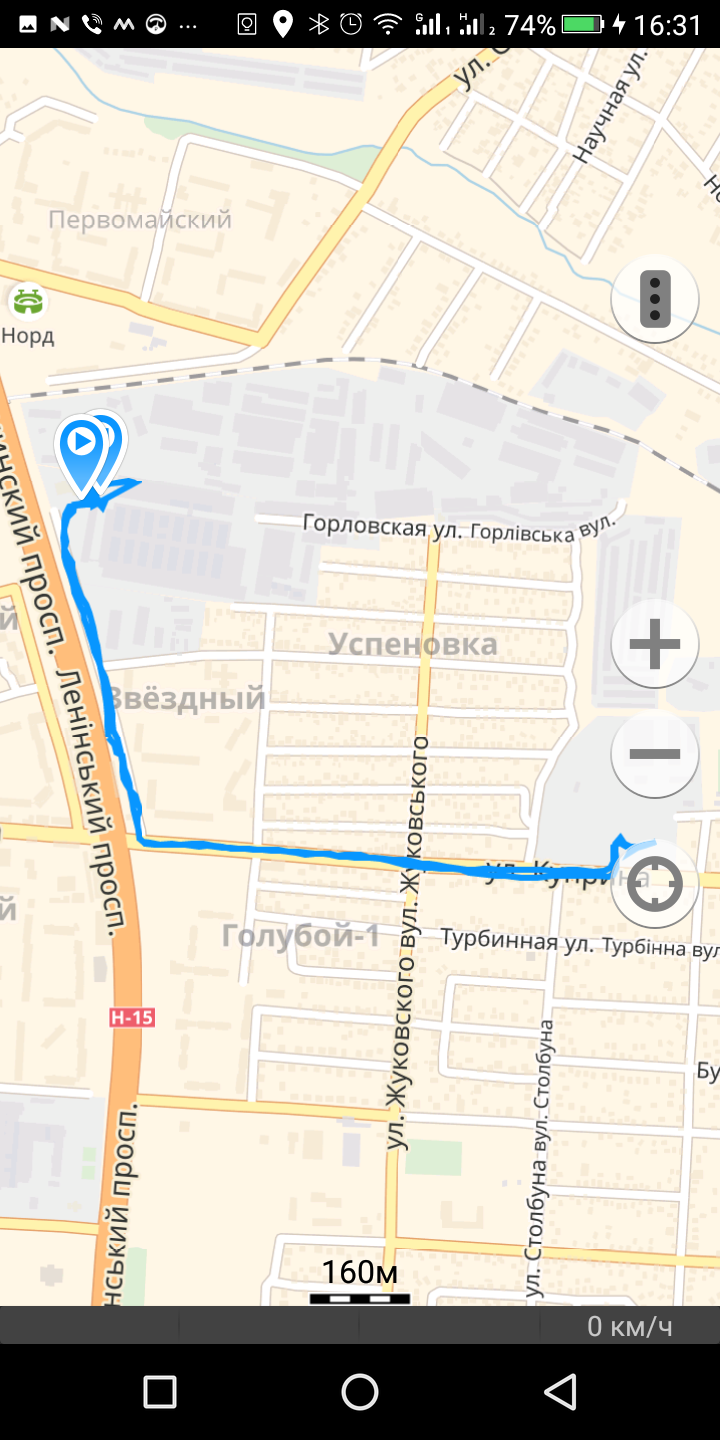
\includegraphics[width=10.94cm]{images/example.png}
	\caption{Пример трекера}
	\label{fig:card}
\end{figure}


%%% Введение                %%%
%%%                         %%%
%%%%%%%%%%%%%%%%%%%%%%%%%%%%%%%

\pagebreak
%%%%%%%%%%%%%%%%%%%%%%%%%%%%%%%%
%%%                          %%%
%%% Обзор                    %%%

%%% В обзоре раскрывается текущее состояние исследований/разработок    %%%
%%% в выбранной Вами области                                           %%%

\section{Обзор приложений в данной области}

\subsection{Spyzie}

Spyzie является полным устройство слежения приложения ,
 которое позволит вам получить доступ к существенной информации , 
 относящейся к устройству в одном месте. Очень проста в использовании, 
 имеет веб-интерфейс для пользователя панель управления , которая может быть 
 доступна практически на любом устройстве. Приложение может быть использовано для 
 получения обновления местоположения в режиме реального времени и 
 позволяет доступ важных данных (например , сообщения, фотографии, заметки и многое другое) на устройстве.\cite{review5}
 \begin{figure}
 	\centering
 	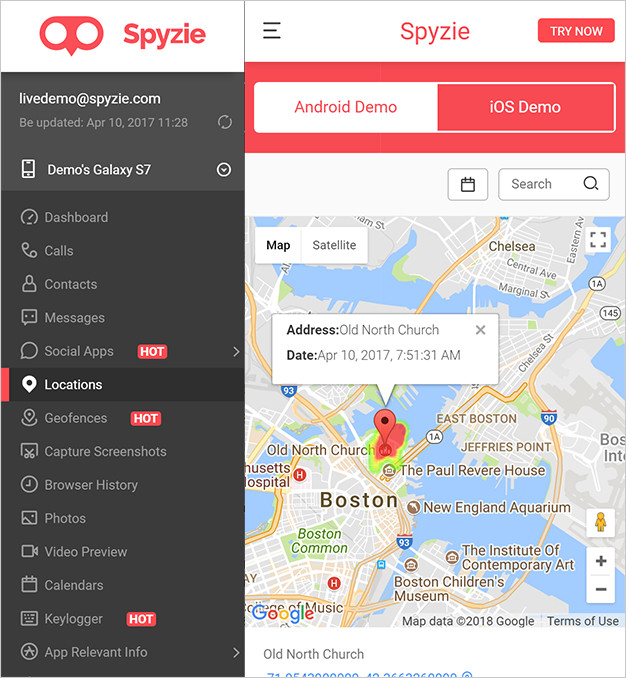
\includegraphics[width=10.94cm]{images/spy-location.jpg}
 	\caption{Spyzie}
 	\label{fig:card}
 \end{figure}
\subsection{Жизнь 360}
Жизнь 360 является полной семьей отслеживания приложения , которое поставляется с большим количеством дополнительных функций. Вы можете легко добавить круги для вашей семьи и друзей , чтобы знать свои последние места. С его помощью вы также можете получить журнал своих прошлых мест , а также. Это один из лучших Android приложений GPS трекер, который поставляется с дополнительной поддержкой вождения. Он может обнаружить сбой, отправить экстренное сообщение, и проанализировать ваш шаблон вождения.\cite{review5}
\begin{figure}
	\centering
	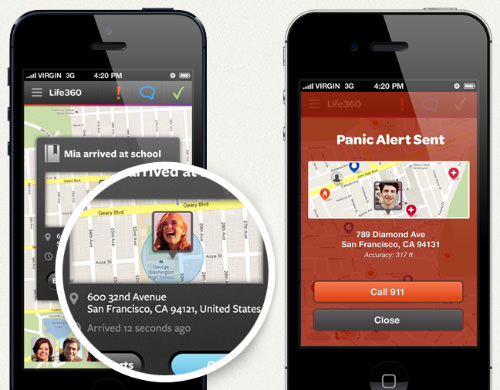
\includegraphics[width=10.94cm]{images/15023617296655.jpg}
	\caption{Жизнь 360}
	\label{fig:card}
\end{figure}
\subsection{GPS Phone Tracker}
GPS Phone Tracker является одним из старейших и наиболее широко используется следящий Android устройства приложений там. То , что делает его одним из лучших следящих приложений Android GPS являются его легко возможности подключения, точные результаты и бесшовные использования. Можно использовать приложение , чтобы получить точное местоположение своих друзей и семьи. Она также имеет функцию отслеживания устройства , чтобы получить обновление в режиме реального времени для потерянного телефона Android.\cite{review5}
\begin{figure}
	\centering
	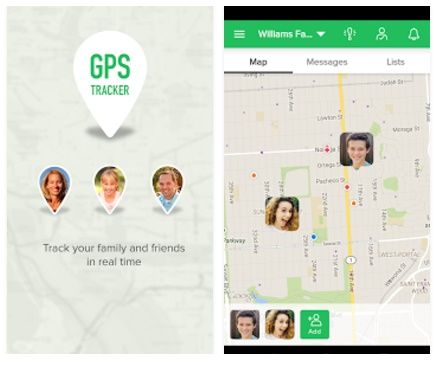
\includegraphics[width=10.94cm]{images/15023616915620.jpg}
	\caption{GPS Phone Tracker}
	\label{fig:card}
\end{figure}
\subsection{Glympse}
Glympse является все-в-один GPS трекер для Android , который будет отслеживать местонахождение без вторжения в вашу частную жизнь. Он может быть использован для отслеживания доставки, запросить местоположение ваших друзей или сообщить своей семье и коллегам о своем местонахождении. Приложение также может быть использовано для отслеживания устройства , чтобы защитить его от кражи.\cite{review5}
\begin{figure}
	\centering
	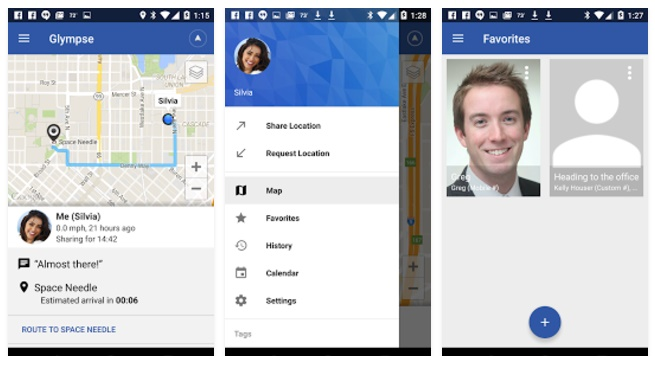
\includegraphics[width=10.94cm]{images/15023616597135.jpg}
	\caption{Glympse}
	\label{fig:card}
\end{figure}
\subsection{Где мой Droid}
Если вы ищете надежный способ , чтобы найти телефон удаленно, то вы должны обязательно дать Где мой Droid попробовать. GPS трекер для Android уже используется миллионами людей во всем мире , чтобы получить в режиме реального времени и точное местоположение своего устройства. Он имеет отличную функцию защиты от кражи с пассивными геоданных и гео-ограждением собственности.\cite{review5}
\begin{figure}
	\centering
	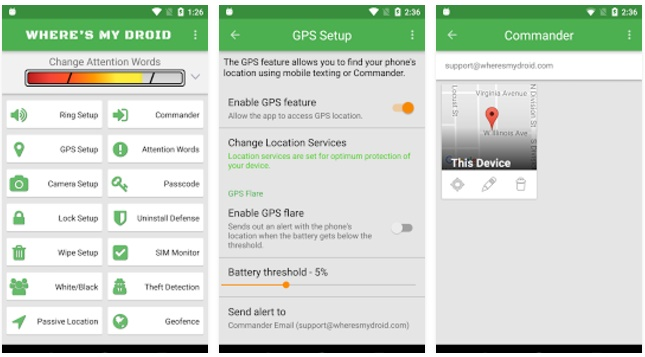
\includegraphics[width=10.94cm]{images/15023616093087.jpg}
	\caption{Где мой Droid}
	\label{fig:card}
\end{figure}

\pagebreak

\section{Алгоритм получение координат}
\subsection{Описание алгоритма}
Приложение запрашивает у android-устройства разрешение на получение
данных о местоположение пользователя. Если оно получено, то
запускается опрос координат с определенным интервалом. С помощью
обработчиков событий можно получить новые координаты, как только они
изменились. Разработчик может выбирать частоту обновления и точность 
местоположения. Они должны быть такими, чтобы приложение было 
энергоэффективным, но при этом погрешность кооординат не была 
слишком большой. Данные о координатах устройство получает с помощью
GPS-модуля или информации о подключении к Интернету.\cite{documentation}
%%% Обзор                   %%%
%%%                         %%%
%%%%%%%%%%%%%%%%%%%%%%%%%%%%%%%

\pagebreak
%%%%%%%%%%%%%%%%%%%%%%%%%%%%%%%%
%%%                          %%%
%%% Постановка задачи        %%%

%%% Итогом этого раздела должна быть ясная формулировка задач, требующих %%%
%%% решения для достижения цели, кратко указанной во введении            %%%

\section{Постановка задачи}

\subsection{Создание трекера пользователя}

Такая серьёзная задача требует знаний и умений в области
разработки приложений под платформу Android. Прежде всего
требуется разработать тестовый вариант приложения, который
позволит оценить расход батареи мобильного устройства. Оно
постоянно работать и опрашивать местоположение пользователя.
Статистика расхода батареи позволит сделать вывод
о возможности создания энергоэффективного трекера.

Для достижения поставленной цели необходимо решить задачи:

\begin{enumerate}
\item Изучить основные принципы разработки мобильного приложения
\item Установить и настроить инструменты разрабодки под платформу Android
\item Изучить основные технологии создания приложений под платформу Android
\item Изучить технологии отслеживания местоположения
\item Изучить технологии работы приложения в фоновом режиме
\item Написать тестовое приложение
\item Написать основное приложение
\end{enumerate}

%%% Постановка задачи        %%%
%%%                          %%%
%%%%%%%%%%%%%%%%%%%%%%%%%%%%%%%%

\pagebreak
%%%%%%%%%%%%%%%%%%%%%%%%%%%%%%%%
%%%                          %%%
%%% Результаты               %%%

%%% Здесь опишите то, что уже сделано на данном этапе %%%

\section{Текущие результаты}

На данный момент получены следдующие результаты:

\begin{enumerate}
\item Изучены базовые принципы разработки мобильных приложений
\item Установлены и настроены инструменты разработки под Android
\item Изучены основные технологии разработки под платформу Android
\item Изучены технологии отслеживания местоположения
\item Написано тестовое приложение без работы в фоне
\end{enumerate}


%%% Пример внутристрочной и выключной формулы %%%


%%% Результаты               %%%
%%%                          %%%
%%%%%%%%%%%%%%%%%%%%%%%%%%%%%%%%
\pagebreak
\section{Приложение}
\subsection{Java-код}
\lstinputlisting[language=Java]{../app/src/main/java/com/beginerdranch/android/myapplication/LocationActivity.java}
\subsection{XML-разметка}
\lstinputlisting{../app/src/main/res/layout/activity_location.xml}
\pagebreak
%%%%%%%%%%%%%%%%%%%%%%%%%%%%%%%%
%%%                          %%%
%%% Использованные источники %%%

\renewcommand{\bibname}{Библиографический список использованной литературы}
\begin{thebibliography}{99}
%\thispagestyle{empty}
\vspace{5mm}
\addcontentsline{toc}{section}{Библиографический список использованной литературы}

\bibitem{review}
Геотрекер - GPS трекер - Всё о пройденном пути [Электронный ресурс] : [сайт] - Электрон. дан. 
- Режим доступа:http://helpix.ru/appinion/201806/2160-geotreker\_-\_gps\_treker-vsjo\_o\_projdennom\_puti.html - Загл. с экрана.

\bibitem{review5}
5 лучших GPS приложения Tracker для Android в 2018 году [Электронный ресурс] : [сайт] - Электрон. дан. 
- Режим доступа:http://global.spyzie.biz/ru/android-tracker/best-gps-tracker-apps-for-android.html - Загл. с экрана.

\bibitem{documentation}
Android Developers [Электронный ресурс] : [сайт] - Электрон. дан. 
- Режим доступа:https://developer.android.com/ - Загл. с экрана.

\bibitem{playmarket}
Google Play [Электронный ресурс] : [сайт] - Электрон. дан. 
- Режим доступа:https://play.google.com - Загл. с экрана.

\bibitem{book}
Филлипс Б., Стюарт К., Марсианко К. {\it Android программирование для профессионалов} М.: Питер. 2017 --- 687 с.

\end{thebibliography}

%%%                          %%%
%%%%%%%%%%%%%%%%%%%%%%%%%%%%%%%%

\end{document}
